\section{Ultrafast jet classification at the HL-LHC}
{{\footnotesize
\begin{description}[labelwidth=5em, labelsep=1em, leftmargin=*, align=left, itemsep=0.3em, parsep=0em]
  \item[date:] 2024-07-08
  \item[last\_updated:] 2024-07
  \item[expired:] unkown
  \item[valid:] yes
  \item[url:] \href{https://arxiv.org/pdf/2402.01876}{https://arxiv.org/pdf/2402.01876}
  \item[domain:] Particle Physics
  \item[focus:] FPGA-optimized real-time jet origin classification at the HL-LHC
  \item[keywords:]
    - jet classification
    - FPGA
    - quantization-aware training
    - Deep Sets
    - Interaction Networks
  \item[task\_types:]
    - Classification
  \item[ai\_capability\_measured:]
    - Real-time inference under FPGA constraints
  \item[metrics:]
    - Accuracy
    - Latency
    - Resource utilization
  \item[models:]
    - MLP
    - Deep Sets
    - Interaction Network
  \item[ml\_motif:]
    - Real-time
  \item[type:] Model
  \item[ml\_task:] Supervised Learning
  \item[notes:] Uses quantization-aware training; hardware synthesis evaluated via hls4ml
  \item[contact.name:] Patrick Odagiu
  \item[contact.email:] unkown
  \item[dataset.name:] Zenodo DOI:10.5281/zenodo.3602260
  \item[dataset.url:] \href{constituent-level jets}{constituent-level jets}
  \item[results.name:] ChatGPT LLM
  \item[results.url:] \href{https://docs.google.com/document/d/1gDf1CIYtfmfZ9urv1jCRZMYz\_3WwEETkugUC65OZBdw}{https://docs.google.com/document/d/1gDf1CIYtfmfZ9urv1jCRZMYz\_3WwEETkugUC65OZBdw}
  \item[fair.reproducible:] True
  \item[fair.benchmark\_ready:] False
  \item[ratings.software.rating:] 0
  \item[ratings.software.reason:] Not analyzed. 
  \item[ratings.specification.rating:] 8.0
  \item[ratings.specification.reason:] Task is clear (RL control of beam stability), with BOOSTR-based simulator; control objectives are well motivated, but system constraints and reward structure are still under refinement.
  \item[ratings.dataset.rating:] 7.0
  \item[ratings.dataset.reason:] BOOSTR dataset exists and is cited, but integration into the benchmark is in early stages; metadata and FAIR structure are limited.
  \item[ratings.metrics.rating:] 7.0
  \item[ratings.metrics.reason:] Stability and control loss are mentioned, but metrics are not yet formalized with clear definitions or baselines.
  \item[ratings.reference\_solution.rating:] 5.5
  \item[ratings.reference\_solution.reason:] DDPG baseline mentioned; PPO planned; implementation is still in progress with no reproducible results available yet.
  \item[ratings.documentation.rating:] 6.0
  \item[ratings.documentation.reason:] GitHub has a defined structure but is incomplete; setup and execution instructions for training/evaluation are not fully established.
  \item[id:] ultrafast\_jet\_classification\_at\_the\_hl-lhc
  \item[Citations:] \cite{odagiu2024ultrafastjetclassificationfpgas}
  \item[Ratings:]
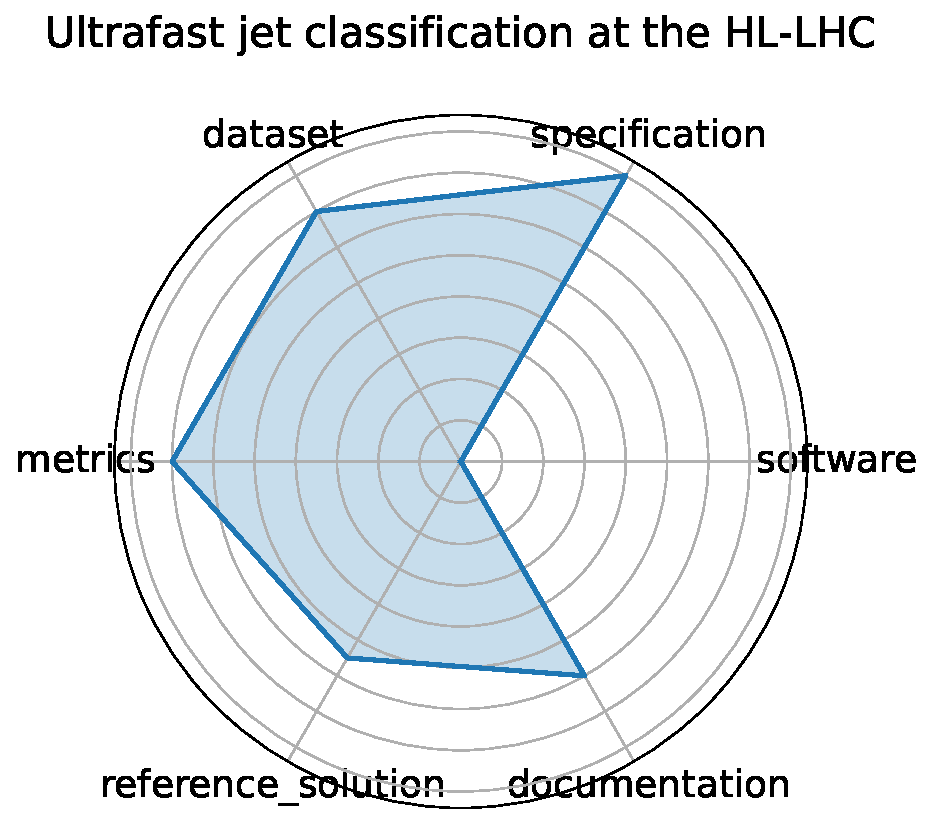
\includegraphics[width=0.2\textwidth]{ultrafast_jet_classification_at_the_hl-lhc_radar.pdf}
\end{description}
}}
\clearpage